\begin{figure}[!ht]
	\centering
	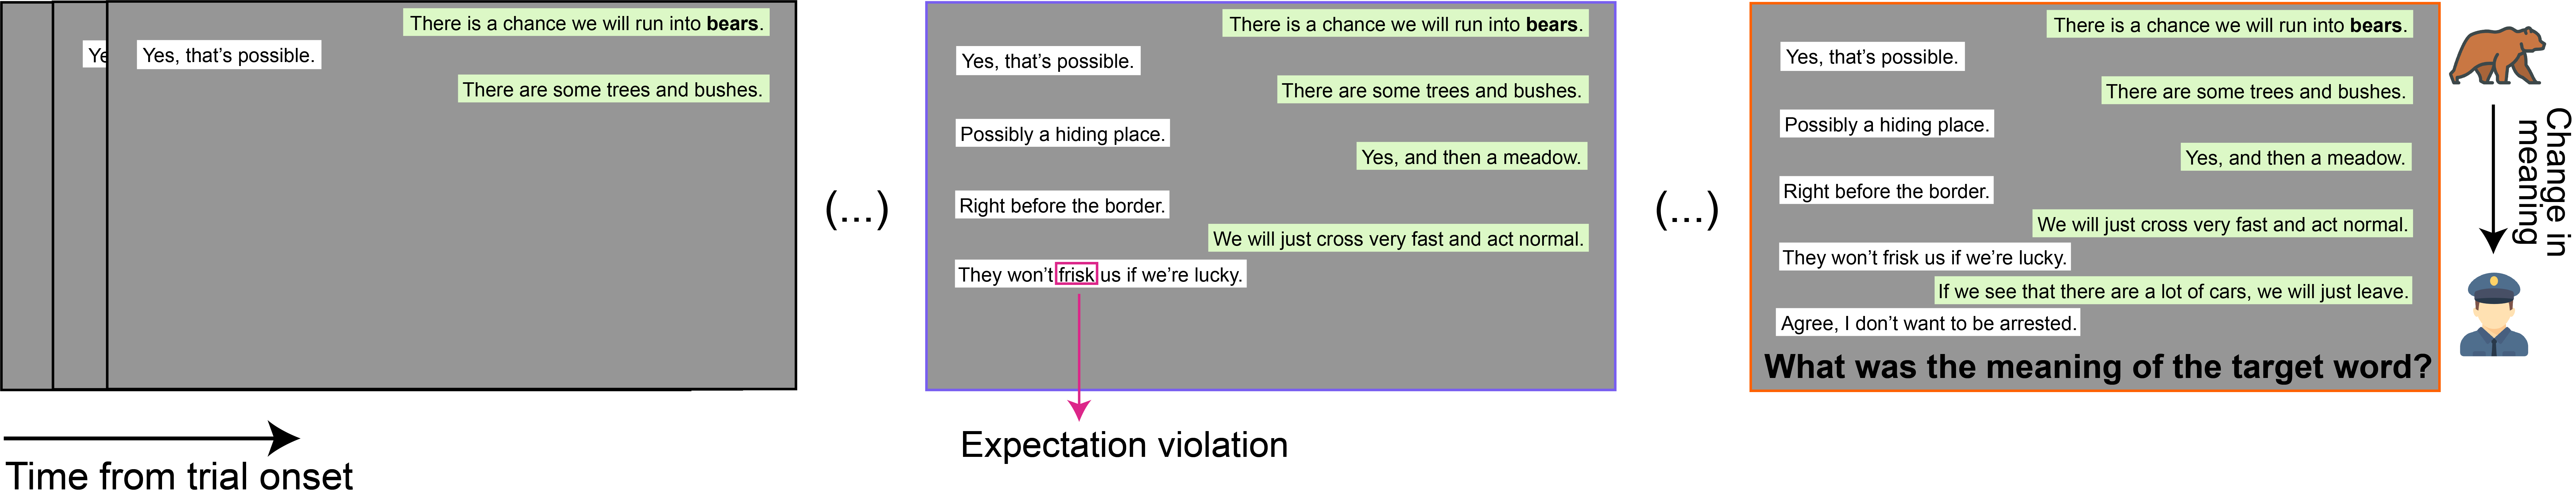
\includegraphics[width=.9\textwidth, clip=true]{./Chapters/06_Discussion/Images_MM/csi_image_horizontal}
	\caption{The NeuroCSI paradigm, which aims to probe the cognitive processes underlying the integration of context with utterance meaning. Participants read the chat conversation for which sentences appear on screen one at a time. In this example trial, the target word (\textit{bears}) has a different meaning (\textit{police}) than its literal meaning. The first sentence that could indicate that the target word has a slang meaning is the \textit{expectation violation} (see screen with purple outline), a critical event for analysis. After all sentences have appeared on screen, the participants decide on the meaning of the target word (see screen with orange outline). In these "slang" trials, the likely meaning of the target word has changed from its literal meaning to the slang meaning over the course of the dialogue and can be inferred from the context. }
    \vspace*{-10pt}
	\label{fig:csi}
\end{figure}